\documentclass[../main.tex]{subfiles}
\begin{document}

\chapter{里德堡原子阵列中的量子多体疤痕}

\section{引言}
里德堡原子阵列为研究动力学受限多体系统中的量子信息动力学提供了一个可控且可扩展的平台\cite{kumar2018sorting,sheng2022defect,graham2022multi,barnes2022assembly,kim2022rydberg,okuno2022high,chen2023continuous,liu2023realization,singh2023mid,eckner2023realizing,ma2023high,zhao2023floquet,bluvstein2024logical,gregory2024second,pause2024supercharged,shaw2024benchmarking}。在该平台中,里德堡原子之间的强范德瓦尔斯相互作用(vdW),诱导里德堡阻塞机制\cite{lukin2001dipole,urban2009observation_combined},从而抑制相邻格点的同时激发到里德堡态,并对局域量子比特翻转施加动力学约束。在适当参数范围内,系统可由 PXP 哈密顿量近似描述\cite{lesanovsky2012interacting,turner2018weak}:
\begin{equation}
  \hat{H}_\text{PXP} =
  \sum_i\hat{P}_i\hat\sigma^x_{i+1}\hat{P}_{i+2}.\label{Eq:PXP}
\end{equation}
其中,$\hat{P}_i = (1 - \hat\sigma^z_i)/2$ 是格点 $i$ 处自旋向下 $\ket{\downarrow}$ 态的投影算符,$\hat\sigma^{x,y,z}_i$ 为第 $i$ 个自旋的泡利算符。以此为基础的研究揭示了量子多体疤痕这一非遍历动力学结构\cite{bernien2017probing,turner2018weak,serbyn2021quantum,bluvstein2021controlling,desaules2024ergodicity}。进一步的理论工作表明,动力学约束不仅能够支撑疤痕态复苏,还可能带来区别于典型混沌体系的信息加扰行为,从而为时空量子信息动力学的实验检验提供了清晰切入点\cite{yuan2022quantum}。

图~\ref{Fig:1}a 
\todo[inline, color=blue!20]{这里差一张图,}给出了对该类信息传播动力学的直观图像。在 PXP 模型中,以反铁磁尼尔态
$\ket{\mathbb{Z}_2}=
 \ket{\uparrow\downarrow\uparrow\downarrow\uparrow\cdots}
$
为初态时,中心自旋上的局域微扰可编码一比特信息。该微扰在动力学约束下引发相邻自旋的迟滞响应,并以近似弹道形式向外传播,形成近似线性的光锥波前。在光锥内部,自旋在受限子空间内继续相干旋转,但不同初态轨道之间的可分辨性呈现周期性衰减与恢复,其特征可由 $\hat\sigma^y$ 期望值差异的演化刻画(虚线圆圈)。这与典型混沌量子系统形成对比:后者光锥内部的局域信息通常会快速扩散并变得不可分辨。由此,动力学受限体系可能表现出持续的信息回流以及对量子混沌的非平凡抑制,为实验探测独特的信息加扰动力学提供了可操作的路径\cite{yuan2022quantum}。

\section{实验方案}
\todo[inline, color=blue!20]{这里应该需要一节,用于更加详细地介绍量子多体疤痕态的内容,以及我们的实验方案。但是第五章只是为了第六章用OTOC和Holevo研究做铺垫,完全不涉及具体的实验方案,就比较头疼。感觉引言的最后一段需要扩展一点,说明高效的量子疤痕态制备和精准地控制动力学受限体系的演化,是后两章研究的基础,所以这里需要单独开辟一章进行描述,当作后两章的前置工作。应该甚至可以多放点量子疤痕态的理论部分,介绍能级结构啥的。}

\section{实验装置与控制}

\subsection{实验方法概述}

\subsubsection{无缺陷原子阵列的制备}
在本文实验中,原子从磁光阱加载,并由经空间光调制器(Spatial Light Modulator, SLM)衍射的聚焦 808-\unit{nm} 激光束形成的光镊俘获。通过“测量—反馈—重排”的闭环过程,本文消除了原子链中的缺陷,实现了全填充阵列的快速制备(图~\ref{Fig:extended_1}a)。

\subsubsection{实验参数}
制备无缺陷阵列后,原子被光抽运到基态。原子间距约为 \SI{7}{\um},对应最近邻与次近邻相互作用强度分别为 $V_{i,i+1} = 2\pi \times \SI{7.3}{MHz}$ 和 $V_{i,i+2} = 2\pi \times \SI{0.11}{MHz}$。为了在固定的 vdW 相互作用比值 $V_{i,i+1} / V_{i,i+2} \approx 64$ 下尽可能逼近 PXP 模型,本文在演化过程中选取基态—里德堡驱动拉比频率 $\Omega = V_{i,i+1}/6 = 2\pi \times \SI{1.21(1)}{\MHz}$,并引入小失谐 $\Delta =2\pi\times\SI{0.22(1)}{\MHz}$ 以补偿残余的次近邻相互作用 $V_{i,i+2}$。在该参数下,实验里德堡哈密顿量可被 PXP 模型很好地近似,数值模拟表明由长程项引入的偏差在本文关心的时间尺度内可忽略(详见第~\ref{section:experimental-parameter} 节)。

\subsubsection{高保真度 $\ket{\mathbb{Z}_2}$ 态制备}
795-\unit{\nano\meter} 与 480-\unit{\nano\meter} 寻址激光束由 SLM 衍射产生,并通过高数值孔径物镜聚焦到原子上。通过调节 SLM 相位全息图实现格点选择性寻址。795-\unit{\nano\meter} 寻址光束非共振耦合 $\ket{5S_{1/2}}$ 基态到 $\ket{5P_{1/2}}$ 态(图~\ref{Fig:extended_1}b),在被寻址原子上诱导光频移。在 $\ket{\mathbb{Z}_2}$ 态制备期间,被寻址原子经历 $2\pi \times \SI{12.2(3)}{MHz}$ 的光频移,从而有效屏蔽其里德堡激发。结合高保真度全局基态-里德堡态 $\pi$ 脉冲,本文实现了多达 25 个原子的 $\ket{\mathbb{Z}_2}$ 有序阵列制备(图~\ref{Fig:2}b)。

\begin{figure}[htb]
  \centering
  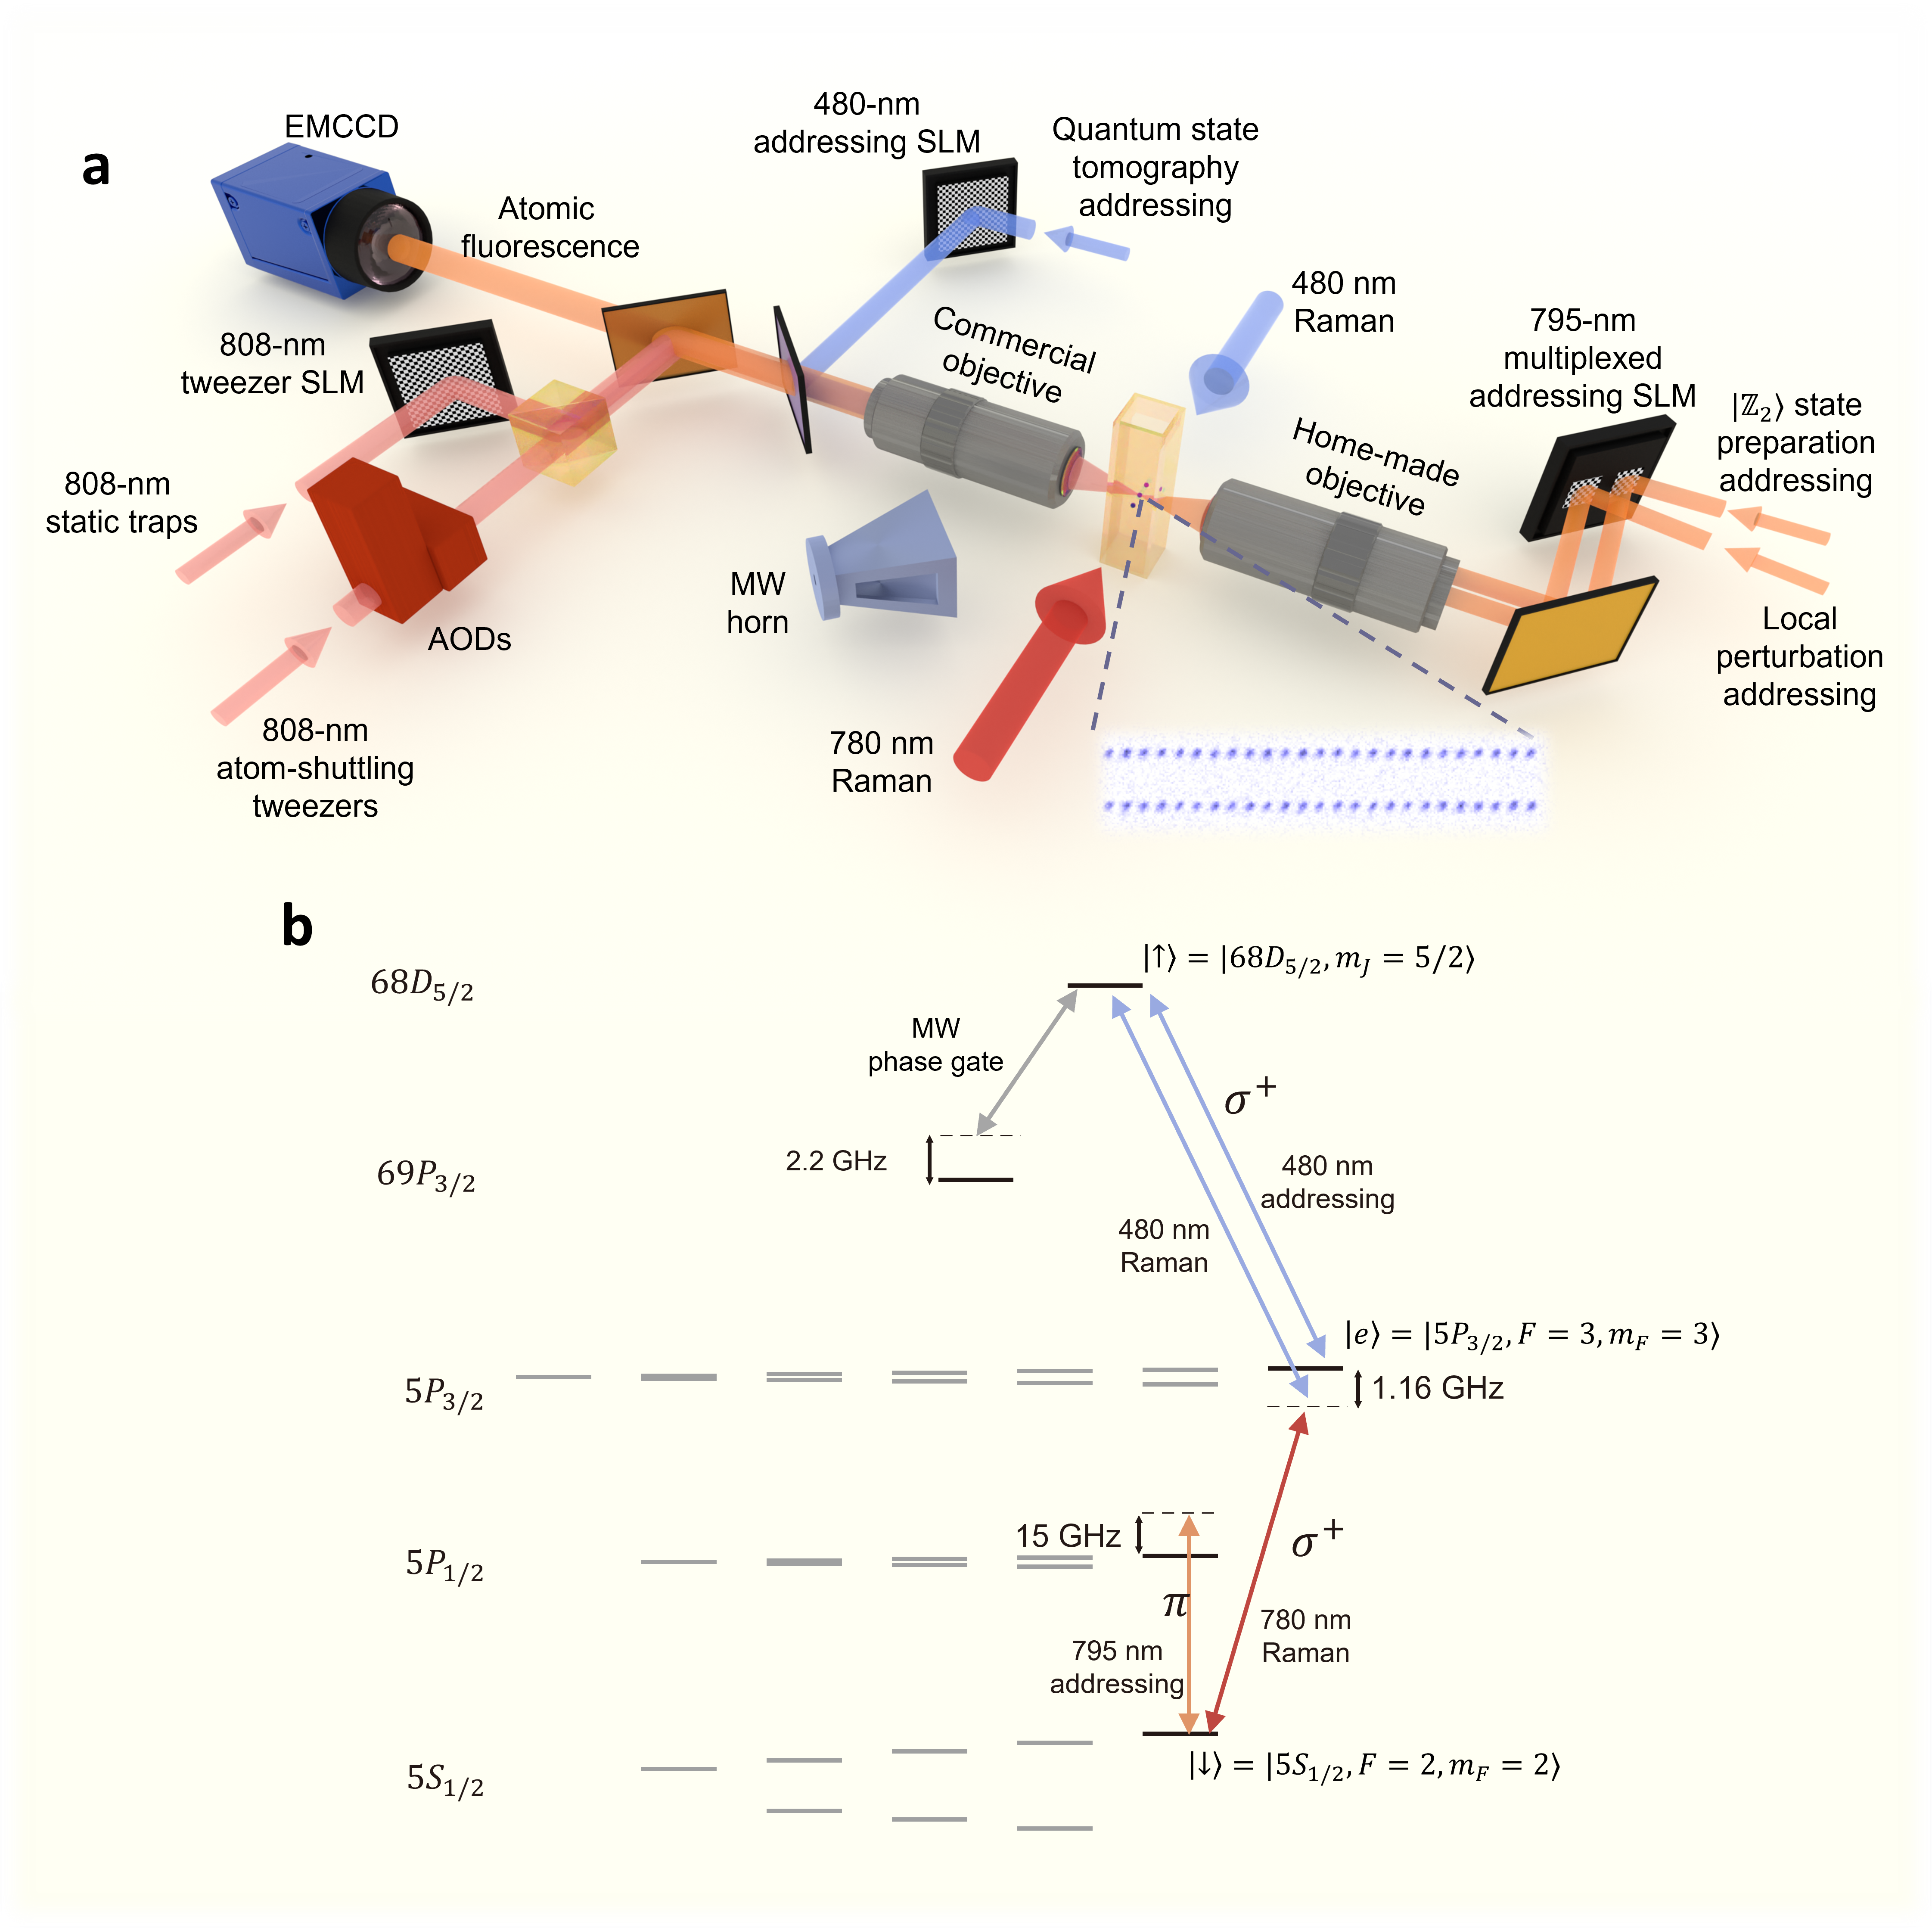
\includegraphics[width=0.7\textwidth]{chapters/chapter_06/figure/Extended_Fig_1.png}
  \caption{
    \textbf{实验装置和原子能级图。} 
    \textbf{a}, 实验装置中基本元件示意图。808-nm 静态光镊由 SLM 产生,原子运输光镊由两个声光偏转器(Acousto-Optic Deflector, AOD)控制。480-\unit{\nano\meter} 寻址激光束由另一个 SLM 产生。商业物镜 (G Plan Apo 50$\times$, Mitutoyo, NA = 0.5) 聚焦 808-nm 光镊光束和 480-\unit{\nano\meter} 寻址光束,同时收集 795-\unit{\nano\meter} 原子荧光用于电子倍增 CCD(EMCCD)相机成像。反向传播的 780-\unit{\nano\meter} 和 480-\unit{\nano\meter} 拉曼光束实现相干基态—里德堡操控。用于局域微扰 \(\hat\sigma_c^z\) 的 795-\unit{\nano\meter} 寻址激光与负责产生交替光频移图案的激光阵列瞄准同一 SLM 的不同区域,通过空间复用实现亚微秒级切换。腔体附近的微波喇叭产生用于里德堡态操控(相位门)与探测的微波脉冲。插图显示原子阵列。
    \textbf{b}, $^{87}$Rb 原子能级图。本文采用从基态 \(\ket{\downarrow} = \ket{5S_{1/2}, F=2, m_F=2}\) 到里德堡态 \(\ket{\uparrow} = \ket{68D_{5/2}, m_J=5/2}\) 的双光子拉曼跃迁。该跃迁由 \(\hat\sigma^+\) 偏振的 780-\unit{\nano\meter} 激光(耦合基态到中间态 \(\ket{e}=\ket{5P_{3/2}, F=3, m_F=3}\))和 \(\hat\sigma^+\) 偏振的 480-\unit{\nano\meter} 激光(连接中间态到里德堡态)驱动,两束激光相对于中间态失谐 \(\Delta = 2\pi\times\SI{1.16}{\giga\hertz}\)。微波场相对于 \(\ket{\uparrow}\rightarrow\ket{69P_{3/2}, m_J=3/2}\) 跃迁红失谐 $2\pi\times\SI{2.2}{\giga\hertz}$,在里德堡态上产生交流斯塔克频移,并提供用于反转 PXP 哈密顿量的相位门。局域单量子比特控制采用相对于 \(\ket{\downarrow}\rightarrow\ket{5P_{1/2}}\) 跃迁蓝失谐 $2\pi\times\SI{15}{\giga\hertz}$ 的 795-\unit{\nano\meter} 寻址光束,以及与 \(\ket{\uparrow}\rightarrow\ket{e}\) 跃迁共振的 480-\unit{\nano\meter} 寻址光束。
    }
  \label{Fig:extended_1}
\end{figure}

\section{实验细节}
\label{section:experiment}
{
可编程原子阵列已成为量子模拟与量子计算的关键平台之一,核心优势在于其对阵列几何、局域操控与单原子探测的并行可编程能力。围绕阵列制备~\cite{piotrowicz2013two,endres2016atom,barredo2016atom,lee2017defect,barredo2018synthetic,kumar2018sorting,sheng2022defect,barnes2022assembly,okuno2022high,liu2023realization,pause2024supercharged}、量子计算~\cite{isenhower2010demonstration,jau2016entangling,sheng2018high,omran2019generation,guo2020balanced,bluvstein2022quantum,graham2022multi,fu2022high,schine2022long,singh2023mid,evered2023high,scholl2023erasure,ma2023high,zhao2023floquet,bluvstein2024logical,gregory2024second,shaw2024benchmarking}、量子优化~\cite{graham2022multi,ebadi2022quantum,kim2022rydberg,bluvstein2024logical}、量子模拟~\cite{bernien2017probing,keesling2019quantum,ebadi2021quantum,scholl2021quantum,semeghini2021probing,fang2024probing,DeLeseleuc2019,scholl2022microwave,chen2023continuous,kim2024realization}与量子计量~\cite{bornet2023scalable,eckner2023realizing}的研究均依赖这一能力的持续提升。
\todo[inline, color=blue!20]{上面这几句话应该移到第一章,这里不需要介绍可编程原子阵列这么大的背景}
本文在本节给出实验实现细节,包括实验装置、时序,以及 $\ket{\mathbb{Z}_2}$ 态的制备与表征。
}

\subsection{实验装置}
\label{section:setup}
\todo[inline, color=blue!20]{实验装置这一整节的大部分内容都应该融并到第三章和第四章,唯一需要提及的内容就只有静态光镊阵列的构型和间距,以及795-nm寻址光的产生和打光方式。}
{
本文实验平台围绕双腔真空系统搭建,包括 2D 磁光阱(Magneto-Optical Trap, MOT)腔与科学腔。在 2D-MOT 腔中,$^{87}$Rb 原子源(安瓿)提供扩散原子蒸气,原子由磁场与 780-\unit{\nano\meter} 激光冷却与束缚;冷却光相对于 $\ket{5S_{1/2}, F=2} \rightarrow \ket{5P_{3/2}, F=3}$ 循环跃迁红失谐 $2\pi\times \SI{30}{\MHz}$。预冷原子随后通过差分泵浦孔径由 780-\unit{\nano\meter} 推送光束转移至科学腔。
科学腔为定制长方体玻璃腔 (Japan Cell),其超高真空由非蒸散型吸气剂泵 (NEXTorr D 200-5, SAES) 维持,背景压力低于 \(10^{-11}\) mbar。该条件最初支持超过 \SI{10}{\minute} 的单原子俘获寿命;由于 2D-MOT 腔中离子泵 (SP-4, JJJvac) 故障,寿命降至约 \SI{90}{\second}。科学腔中的原子由三维磁光阱(3D-MOT)捕获与冷却,使用三对反向传播的 780-\unit{\nano\meter} 激光束,磁场梯度为 \SI{0.15}{\tesla\per\cm}。每束光包含相对于循环跃迁红失谐 $2\pi\times \SI{24}{\MHz}$ 的冷却光,以及与 $\ket{5S_{1/2}, F=1} \rightarrow \ket{5P_{3/2}, F=2}$ 跃迁共振的再泵浦光。
}

{
单原子被加载到静态二维光镊阵列中。静态光镊由 808-nm 激光器 (TA pro, Toptica) 自由运行输出,通过加载加权 Gerchberg--Saxton (WGS) 算法生成的相位全息图的 SLM(HED 6010-NIR-080-C, Holoeye)形成。此外,本文使用与静态阵列同源但偏振正交的 808-nm 光束构建原子运输光镊系统,从而实现精确的原子重排。运输光镊由一对正交取向的 AOD(DTSX-400-800.850, AA Opto-Electronic)控制,其射频驱动由双通道任意波形发生器(Arbitrary Waveform Generator, AWG;M4i.6631-x8, Spectrum)产生的独立波形提供。
}

{高数值孔径物镜 (G Plan Apo 50$\times$, Mitutoyo, NA = 0.5) 聚焦静态与可移动光镊并收集原子荧光,荧光被引导到 EMCCD (iXon Ultra 888, Andor) 探测。此外,用于局域里德堡操控的 480-\unit{\nano\meter} 光束也通过同一物镜聚焦(见图~5a)。捕获、寻址与荧光探测共用同一光路,有助于提高系统的长期稳定性。}
{
与 Mitutoyo 物镜相对的是数值孔径为 0.4 的自制物镜。CCD 相机对静态光镊阵列成像,阵列由 36 \(\times\) 2 个光镊组成,间距为 \SI{7}{\um},束腰约为 \SI{0.9}{\um}。通过迭代反馈与调整,阵列强度起伏被压制在 1\% 以内。对于 $\ket{\mathbb{Z}_2}$ 态制备与局域微扰至关重要的 795-\unit{\nano\meter} 寻址光束通过自制物镜聚焦。两束反向传播激光(\SI{780}{\nm} 与 \SI{480}{\nm})实现全局基态—里德堡相干操控。科学腔附近的微波天线提供用于里德堡态操控与探测的微波脉冲。}

{
实验平台集成了用于态制备、量子比特控制与探测的多套激光系统。780-\unit{\nano\meter} 激光系统为锥形放大器激光器 (TA Pro, Toptica),用于 MOT 冷却与里德堡激发方案中的拉曼光,其频率稳定到精细度为 26,000 的超低膨胀参考腔 (SLS)。AWG 驱动针对调制带宽优化的单次通过声光调制器(Acousto-Optic Modulator, AOM;SGT200-780-0.5TA-B),用于动态调节脉冲频率与强度。
为了耦合 \(\ket{e} \rightarrow \ket{r}\) 跃迁,本文使用 480-\unit{\nano\meter} 激光系统(倍频 TA-SHG Pro, Toptica),其 960-nm 种子激光器锁定到与 780-\unit{\nano\meter} 激光器相同的参考腔。由直接数字合成(Direct Digital Synthesis, DDS;AD9910)驱动的 AOM 控制 480-\unit{\nano\meter} 光束的频率与强度,该光束经强度稳定后在里德堡序列中保持开启。里德堡激发光的快速上升与下降沿由电光调制器(Electro-Optic Modulator, EOM)实现,以满足时序切换需求。
}

\begin{figure}
  \centering
  \includegraphics[width=0.7\textwidth]{chapters/chapter_06/figure/SI_Timing_sequence.png}  
  \caption{
    \textbf{实验时序。} 
    本文实验序列的概要见图示。用于 OTOC 与 Holevo 信息测量的详细里德堡序列在图~\ref{SI_OTOC_sequence},\ref{SI_HI_sequence} 中给出。
    }
  \label{Fig:S1}
\end{figure}

\subsection{实验时序} 
\label{section:timing-sequence}
\todo[inline, color=blue!20]{这一节可以保留, 可以把1.3节 实验方法概述融并进来}

{
实验序列起始于在科学腔中制备冷原子系综。3D-MOT 加载 \SI{200}{\ms},产生直径约 \SI{500}{\um}、温度约 \SI{150}{\micro\kelvin} 的原子云,并通过飞行时间(Time of Flight, TOF)膨胀测量表征。为进一步降低温度,本文采用偏振梯度冷却(Polarization Gradient Cooling, PGC):在 \SI{500}{\us} 内快速关断磁场梯度,同时将冷却光失谐增至约 $2\pi\times\SI{90}{\MHz}$ 并降低冷却与再泵浦光强。该过程将温度降至约 \SI{40}{\micro\kelvin}。
}
{
激光冷却原子系综作为随机加载可编程原子阵列的原子库。随机加载阶段使用两束反向传播的 795-\unit{\nano\meter} 光束实施 \(\Lambda\) 增强灰光学粘团(\(\Lambda\)GM),并辅以针对阱内冷却优化的额外 PGC 阶段。组合冷却使单原子加载效率达到约 80\%,在阱深 \SI{1}{\milli\kelvin} 时平均温度约为 \SI{15}{\micro\kelvin}(由释放—再捕获 (R\&R) 方法测量)。原子荧光探测复用 \(\Lambda\)GM 的 795-\unit{\nano\meter} 光束,并在将阱深提升至 \SI{1.3}{\milli\kelvin} 后进行。在 \SI{30}{\ms} 曝光下,本文实现了超过 99.9\% 的探测保真度,同时将每次探测的平均原子损失控制在 1\% 以下。使用 795-\unit{\nano\meter} 荧光成像可降低强 780-\unit{\nano\meter} 光束引入的串扰,从而提高探测的可靠性。
}

{
原子重排过程用于生成无缺陷一维原子链。该过程起始于将可移动光镊强度从零线性提升至静态阱深的三倍,使原子从静态 SLM 生成的阱转移到可移动光镊。随后通过含时波形驱动 AOD,以平均速度 \SI{100}{\um\per\ms} 运输原子,并采用正弦速度分布以平滑加速与减速。重排路径由改进的匈牙利算法确定\cite{lee2017defect},并按列逐步优化原子移动。为降低运输光镊扫过静态阱时引入的原子损失与加热,路径中包含绕开中间阱的额外段。所有 AOD 波形均为预计算,从而保证重排过程的快速执行。重排后测得原子温度升至约 \SI{50}{\micro\kelvin}。
}

{
相干里德堡激发采用双光子拉曼方案。具有 \(\sigma^+\) 偏振的红失谐 780-\unit{\nano\meter} 光将基态耦合到中间态 \(\ket{5P_{3/2}, F=3, m_F=3}\)(见图~5b)。准直的 780-\unit{\nano\meter} 光束腰约为 \SI{300}{\um},对应最大拉比频率约为 \(\sim 2\pi\times\SI{100}{\MHz}\)。具有 \(\sigma^+\) 偏振的蓝失谐 480-\unit{\nano\meter} 光将中间态耦合到里德堡态 \(\ket{\uparrow} = \ket{68D_{5/2}, m_J=5/2}\),其聚焦束腰为 \SI{13}{\um},最大拉比频率约为 \(\sim 2\pi\times\SI{70}{\MHz}\)。两束光相对于中间态的共同失谐为 \(\Delta = 2\pi\times\SI{1.16}{\GHz}\)。整个实验过程中施加 \SI{3}{\micro\tesla} 的偏置磁场。
图~\ref{SI_Block_Rabi}a(蓝色圆圈)给出单原子在 780-\unit{\nano\meter} 与 480-\unit{\nano\meter} 光驱动下的高对比度基态—里德堡拉比振荡;当两个原子位于阻塞区域内且满足 $\Omega \ll V$ 时,双里德堡激发被显著抑制(黄色方块)。阻塞条件下,单激发子空间中的集体增强使贝尔态 $\frac{1}{\sqrt{2}}(\ket{\downarrow}\ket{\uparrow}+\ket{\uparrow}\ket{\downarrow})$ 与 $\ket{\downarrow}\ket{\downarrow}$ 之间的拉比频率增强 \(\sqrt{2}\) 倍(红色菱形)。图~\ref{SI_Block_Rabi}b 展示单原子的基态—里德堡 Ramsey 相干性:本文执行两次 \(\pi/2\) 旋转并改变间隙时间,Ramsey 条纹衰减给出基态—里德堡相干时间 $T^*_2=\SI{11(1)}{\us}$。该相干性为后续高保真度操作提供基础。
}

\begin{figure}[htb]
  \centering
  \includegraphics[width=0.7\textwidth]{chapters/chapter_06/figure/SI_Block_Rabi.png}  
  \caption{
\textbf{基态-里德堡态拉比振荡、里德堡阻塞和 Ramsey 相干性。} 
{
\textbf{a}, 单原子在 480-\unit{\nano\meter} 与 780-\unit{\nano\meter} 拉曼光驱动下的基态—里德堡拉比振荡(蓝色圆圈)。对于阻塞半径内的一对原子,双里德堡激发被强烈抑制(黄色方块);里德堡阻塞导致单激发子空间中的拉比频率增强 \(\sqrt{2}\) 倍(红色菱形)。曲线为阻尼正弦拟合。
\textbf{b}, Ramsey 条纹的衰减反映高斯型非均匀退相,相干时间为 \(T^*_2 = \SI{11(1)}{\micro\second}\)。测得概率对应 \(\frac{1}{2}(\langle \sigma^y \rangle + 1)\)。
}
}
  \label{SI_Block_Rabi}
\end{figure}

{
为实现基态与里德堡态的局域操作,本文采用由 SLM 生成的 795-\unit{\nano\meter} 与 480-\unit{\nano\meter} 寻址光束。795-\unit{\nano\meter} 光相对于 \(\ket{5S_{1/2}, F=2} \rightarrow \ket{5P_{1/2}}\) 跃迁蓝失谐 \(2\pi \times \SI{15}{\GHz}\),在基态上产生 \(2\pi \times \SI{12.2(3)}{\MHz}\) 的光频移,从而形成可激发与不可激发格点的交替图案,使系统可被制备在 $\mathbb{Z}_2$ 有序配置。本文在 EMCCD 上同时成像 795-\unit{\nano\meter} 原子荧光与寻址光束,以校准激光与原子位置的空间重叠;测量显示对相邻格点的串扰低于 \(2\pi \times \SI{1}{\kHz}\)。
与 $\ket{r}\rightarrow\ket{e}$ 跃迁共振的 480-\unit{\nano\meter} 寻址光束用于选择性里德堡—基态转移,并在最近邻与次近邻格点建立电磁感应透明(Electromagnetically Induced Transparency, EIT)条件。通过最大化目标格点转移效率并最小化相邻格点串扰进行对准优化后,目标格点中超过 96\% 的里德堡布居被快速转移到基态,而相邻格点的里德堡布居减少不到 1\%。
}

{
态探测用于区分基态与里德堡态。在里德堡操作后 \SI{1}{\us} 内,阱深迅速提升至 \SI{1.3}{\milli\kelvin} 以将里德堡原子从捕获区域排出,同时重新捕获基态原子。随后施加扫描强度为 \SI{2.4}{\GHz} 的微波脉冲以耗尽剩余里德堡布居,从而将里德堡原子误识别为基态的概率压低至 1\% 以下。
}

\section{$\mathbb{Z}_2$ 疤痕态的高保真制备}
\subsection{$\ket{\mathbb{Z}_2}$ 态制备和表征}
\label{section:Z2}

\begin{figure}[htb]
  \centering
  \includegraphics[width=0.7\textwidth]{chapters/chapter_06/figure/SI_Z2.png}  
  \caption{
    \textbf{$\ket{\mathbb{Z}_2}$ 态制备细节。} 
    \textbf{a}, 被寻址(红色)与未寻址(蓝色)原子的里德堡激发光谱,里德堡布居随拉曼激发失谐变化。
    \textbf{b}, 反阻塞效应与寻址光诱导光频移对态制备保真度的影响。数值模拟给出 $\ket{\mathbb{Z}_2}$ 态制备保真度随 795-\unit{\nano\meter} 寻址光频移(以拉比频率 $\Omega$ 为单位)的变化,并比较不同系统尺寸;最近邻里德堡相互作用强度取 $V_{i,i+1}=3\Omega$。红星标记本文实验条件。
    \textbf{c}, $\ket{\mathbb{Z}_2}$ 态制备保真度随系统尺寸变化。红线与蓝线分别为校正与未校正保真度的指数拟合;黄线给出本文寻址方法的理论上限。
    \textbf{d}, 13 量子比特微观态出现次数的统计(共 1,774 次实验),其中成功制备 $\ket{\mathbb{Z}_2}$ 态 1,246 次(占 70\%)。
    \textbf{e}, 13 量子比特微观态的测量分布,插图给出主要错误态。
  }
  \label{Fig:S2}
\end{figure}

{
遍历量子多体系统通常表现为快速热化\cite{deutsch1991quantum,srednicki1994chaos,rigol2008thermalization,deutsch2018eigenstate,lewis2019dynamics}。在里德堡原子阵列中,多体疤痕态提供了弱破坏遍历性的一类动力学结构\cite{bernien2017probing,turner2018weak,choi2019emergent,ho2019periodic,bluvstein2021controlling,turner2021correspondence,serbyn2021quantum},其特征是在延长时标上保留相干振荡。类似现象也在超导处理器与玻色-哈伯德量子模拟器中被观察到\cite{zhang2023many,su2023observation},并推动了进一步的理论研究\cite{maskara2021discrete,dong2023disorder,liu2024novel,desaules2024ergodicity,aron2024quantum}。
基于对动力学受限体系的分析,理论工作预测:当以 $\mathbb{Z}_2$ 有序尼尔态作为研究 OTOC 与 Holevo 信息时空演化的初态时,可能观察到持续的信息回流以及对量子混沌的非平凡破坏\cite{yuan2022quantum}。因此,高保真度制备 $\ket{\mathbb{Z}_2}$ 初态是后续量子信息动力学实验的关键前提。
本文使用两类初态研究量子信息加扰:(1) $\mathbb{Z}_2$ 有序态 \(\ket{\mathbb{Z}_2} = \ket{\uparrow \downarrow \uparrow \downarrow \uparrow...}\);(2) 平凡直积态 \(\ket{\mathbf{0}} = \ket{\downarrow \downarrow \downarrow \downarrow \downarrow...}\)。其中 \(\ket{\mathbf{0}}\) 可由光抽运直接获得,而在大规模系统中实现高保真度的 \(\ket{\mathbb{Z}_2}\) 态制备仍具有挑战。
先前研究已通过绝热态转移在一维与二维阵列中制备 \(\ket{\mathbb{Z}_2}\) 态\cite{bernien2017probing,omran2019generation,bluvstein2021controlling},其核心是将设计哈密顿量的基态从 \(\ket{\mathbf{0}}\) 绝热演化到 \(\ket{\mathbb{Z}_2}\)。然而,系统尺寸增大时希尔伯特空间维数指数增长并导致能隙变小,从而使绝热路径的制备保真度迅速下降。
}

{
本文采用可扩展的态制备方案,将全局里德堡激发与格点选择性激光寻址结合。SLM 在原子阵列上写入定制光频移图案,使指定格点对基态—里德堡跃迁失谐(图~\ref{Fig:S2}a),从而形成可激发与不可激发原子的交替排列。795-\unit{\nano\meter} 寻址光束相对于 D1 线共振失谐 $2\pi \times \SI{15}{\GHz}$,在基态上诱导 $2\pi \times \SI{12.2(3)}{\MHz}$ 的能级移动,其散射率约为 $2\pi \times \SI{5}{\kHz}$,显著低于拉曼光束引入的散射率。数值模拟(图~\ref{Fig:S2}b)表明,为最大化 \(\ket{\mathbb{Z}_2}\) 态制备保真度,光频移符号需与里德堡相互作用符号相反,以避免反阻塞效应。在本文实验条件下,模拟得到的制备非保真度约为每个量子比特 0.012。
}

{
该方案在系统尺寸扩展时保持良好性能(图~\ref{Fig:S2}c)。制备非保真度主要来自不相关的单量子比特翻转误差:里德堡激发低效率导致每量子比特约 0.8\% 的误差,有限能量移动引入每量子比特约 1.2\% 的误差,探测误差则包括 1\% 的 $\ket{\downarrow}\rightarrow\ket{\uparrow}$ 与 0.5\% 的 $\ket{\uparrow}\rightarrow\ket{\downarrow}$ 误判。该误差分解突出了本文方案相对绝热转移协议的可扩展性。对于多达 25 个原子的阵列,本文实现的 $\ket{\mathbb{Z}_2}$ 态测量保真度为 49(3)\%,探测误差校正后为 60(3)\%。在 $2^{25}$ 维希尔伯特空间中获得该保真度水平,为后续量子信息动力学测量提供了必要的初态质量保障。
}

{
对实验制备的 $\ket{\mathbb{Z}_2}$ 态微观态分布的分析显示误差出现具有非泊松特征(图~\ref{Fig:S2}d)。图~\ref{Fig:S2}e 给出的测量分布表明主要误差通道为 $\ket{\uparrow}\rightarrow\ket{\downarrow}$ 的单量子比特翻转,这与本文态制备基于单量子比特操作的设计一致。该类可预测误差分布有助于对 $\ket{\mathbb{Z}_2}$ 态下的量子信息加扰实验数据实施误差缓解(见第~\ref{section:error} 节)。
}

\section{动力学受限系统中的弱热化观测}

\subsection{动力学受限自旋动力学}

\begin{figure}[htb]
  \centering
  \includegraphics[width=0.7\textwidth]{chapters/chapter_06/figure/Z2.png}
  \caption{
\textbf{态制备与动力学受限多体态演化。} 
\textbf{a}, 在全局相干驱动下,795-\unit{\nano\meter} 寻址的原子(红色)保持静止,而未寻址原子(蓝色)表现出基态—里德堡拉比振荡。
\textbf{b}, $\ket{\mathbb{Z}_2}$ 态制备保真度 $\mathcal{F}_{\mathbb{Z}_2}$ 随系统尺寸变化。
\textbf{c}, 测量的 25 量子比特 $\ket{\mathbb{Z}_2}$ 态的格点分辨里德堡概率 $P_i(\uparrow)$。上图为原子荧光成像,红圈标记里德堡原子。
\textbf{d}--\textbf{g}, 动力学受限多体动力学。\textbf{d} 与 \textbf{f} 分别给出从初态 $\ket{\mathbb{Z}_2}$ 与 $\hat\sigma^x_c\ket{\mathbb{Z}_2}$ 出发时,测得的格点分辨里德堡概率 $P_i(\uparrow)$ 随演化时间的变化。\textbf{f} 中的线性光锥结构起源于边界效应(见第~\ref{section:boundary} 节)。\textbf{e} 与 \textbf{g} 为相应数值模拟结果。模拟采用完整里德堡哈密顿量,并基于噪声源表征引入实验噪声(见方法与补充材料第~4.3~节)。\textbf{d}--\textbf{g} 中红色虚线曲线标记传播波前,\textbf{f} 与 \textbf{g} 中蓝色虚线标记线性光锥。}
  \label{Fig:2}
\end{figure}

\noindent
如图~\ref{Fig:1}b,c 所示,本文量子模拟器由多达 25 个被光镊俘获的单个 $^{87}$Rb 原子构成的一维线性阵列组成。量子比特态 $\ket{\downarrow}$ 与 $\ket{\uparrow}$ 分别编码在原子基态 $\ket{g}$ 与里德堡态 $\ket{r}$ 中。系统由如下哈密顿量支配:
\begin{equation}
\label{eq:rydberg-hamiltonian-main}
  \hat{H}_\text{R}=
  \frac{\Omega}{2}\sum_i\hat\sigma^x_i-
  \Delta\sum_i\hat{n}_i+
  \sum_{i<j}V_{ij}\hat{n}_i\hat{n}_j,
\end{equation}
其中 $\Omega$ 为拉比频率,$\Delta$ 为失谐,$\hat{n}_i = \ket{\uparrow_i}\bra{\uparrow_i}$ 为向 $\ket{\uparrow_i}$ 的投影算符,$V_{ij} \propto 1/R^6_{ij}$ 表示格点 $i$ 与 $j$ 间距 $R_{ij}$ 下的范德瓦尔斯相互作用强度。在 \(V_{i,i+2} \ll \Omega \ll V_{i,i+1}\) 的参数区域,里德堡阻塞抑制相邻格点的同时激发,使该系统可由式~(\ref{Eq:PXP}) 的 PXP 模型近似描述。

高保真度初态制备是后续实验成功的关键。本文通过全局里德堡激发光(\SI{780}{nm} 与 \SI{480}{nm})结合格点选择性 795-\unit{\nano\meter} 寻址光来制备 $\ket{\mathbb{Z}_2}$ 态:寻址光使被寻址原子对基态—里德堡跃迁失谐,从而形成交替的可激发/不可激发图案(图~\ref{Fig:2}a)。如图~\ref{Fig:2}b,c 所示,本文实现了较高的 $\ket{\mathbb{Z}_2}$ 态制备保真度:中心 13 个量子比特为 70(1)\%,整个 25 量子比特链为 49(3)\%。在探测误差校正后,保真度分别提高至 78(1)\% 与 60(3)\%。在 $2^{25}$ 维希尔伯特空间中获得该初态质量是准确探测动力学受限多体态演化与量子信息动力学的前提。

随后,本文研究引言中所述的动力学受限自旋动力学,重点比较 PXP 哈密顿量下 $\ket{\mathbb{Z}_2}$ 与 $\hat\sigma^x_c \ket{\mathbb{Z}_2}$ 两类自旋配置的演化。对于 $\ket{\mathbb{Z}_2}$ 初态(图~\ref{Fig:2}d),自旋在 PXP 约束下相干旋转并形成近似均匀波前;该同步动力学随后受到边界效应影响,边缘处的动力学差异逐步向内传播并弯曲波前。相较之下,对于 $\hat\sigma^x_c \ket{\mathbb{Z}_2}$ 初态(图~\ref{Fig:2}f),本文观测到清晰的线性光锥结构\cite{surace2020lattice,frerot2018multispeed,Chen2019Finite,kuwahara2020strictly}。光锥外自旋几乎不受中心翻转影响,而光锥内的中心微扰诱导相邻自旋出现迟滞响应并形成弧形传播波前,从而直接反映了 PXP 模型的受限动力学机制。实验数据与数值结果(图~\ref{Fig:2}e,g)之间的一致性表明该里德堡量子模拟器能够可靠捕捉动力学受限体系的核心行为,为进一步研究量子信息动力学奠定实验基础。

{随后,本文进一步表征 $\ket{\mathbb{Z}_2}$ 态的演化与寿命。该动力学在 PXP 哈密顿量 \(H = \sum_i P_i \sigma^x_{i+1} P_{i+2}\)~\cite{lesanovsky2012interacting,turner2018weak,cheng2024emergent} 的正向—反向演化(\(e^{-iHt}\) 后跟 \(e^{iHt}\))与仅正向演化(\(e^{-iHt}\))(图~\ref{Fig:S3})下测量。为表征演化,本文测量里德堡布居 \(P(\uparrow)\)(图~\ref{Fig:S3}a,b)与平均畴壁密度(图~\ref{Fig:S3}c,d)。图~\ref{Fig:S3}a,c 的指数拟合给出正向—反向演化下的衰减率,布居的 $1/e$ 寿命约为 \SI{1.6(1)}{\micro\second},平均畴壁密度的 $1/e$ 衰减时间约为 \SI{1.0(3)}{\micro\second}。该衰减限制了正文图 3f 中原始 ZZ-OTOC 数据的对比度。仅正向演化下,平均畴壁密度(图~\ref{Fig:S3}d)可由阻尼正弦拟合得到约 \SI{1.5(1)}{\micro\second} 的寿命。
{
里德堡布居动力学(图~\ref{Fig:S3}b)采用至多五阶的阻尼傅里叶级数拟合,对应 $1/e$ 衰减时间约为 \SI{2.8(2)}{\us}。
}
此外,第~\ref{section:error} 节中基于图~\ref{Fig:S3}b 数据拟合误差模型以表征驱动场噪声。$\ket{\mathbb{Z}_2}$ 态有限寿命导致传输过程中的整体损失,并反映为正文图 4b 中测得的 Holevo 信息全局衰减。畴壁密度的衰减(图~\ref{Fig:S3}c)与振荡对比度降低(图~\ref{Fig:S3}d)表明无缺陷 $\mathbb{Z}_2$ 有序系统在演化过程中逐步解体为子系统,从而模糊动力学并阻碍量子信息传播。虽然态制备误差可较直接地校正,演化误差的缓解更为复杂;因此,对 $\ket{\mathbb{Z}_2}$ 态衰减率的表征为后续误差缓解策略提供了关键输入。}

{
综上,本文展示了在大规模原子阵列中制备 $\ket{\mathbb{Z}_2}$ 态的可扩展方案。通过全局里德堡激发与格点选择性寻址的结合,本文在多达 25 个量子比特的系统中实现了高保真度初态制备,并对其演化动力学进行了定量表征,为进一步研究疤痕体系中的量子信息加扰提供实验基础。
}

\begin{figure}[htb]
  \centering  
  \includegraphics[width=0.7\textwidth]{chapters/chapter_06/figure/SI_lifetime.png}  
  \caption{
\textbf{PXP 哈密顿量演化下的 $\ket{\mathbb{Z}_2}$ 态动力学。} 
{
\textbf{a} 和 \textbf{b}, 初始化量子比特在 \textbf{a}, 正向—反向演化 \((e^{-iHt}\) 后跟 \(e^{iHt})\) 与 \textbf{b}, 仅正向 \((e^{-iHt})\) 演化期间的 \(\ket{\uparrow}\)(蓝色)与 \(\ket{\downarrow}\)(红色)布居。\textbf{a} 中曲线为指数拟合,而 \textbf{b} 采用至多五阶的阻尼傅里叶级数拟合。
\textbf{c} 和 \textbf{d}, 中心 13 个量子比特在 \textbf{c}, 正向—反向演化与 \textbf{d}, 仅正向演化期间的平均畴壁密度 (DWD)。\textbf{c} 中蓝色曲线为指数拟合,而 \textbf{d} 拟合为阻尼正弦函数。
}
}
  \label{Fig:S3}
\end{figure}

\section{理论建模与数值模拟}

\subsection{有效哈密顿量和数值模拟方法}

{本文实验装置由被光镊俘获的 25 个单原子线性阵列构成。系统动力学由微观哈密顿量支配:
\begin{equation}
H = \sum_i \left[\frac{\Omega}{2} \sigma^x_i - \Delta n_i \right] + \sum_{i<j} V_{ij} n_i n_j,
\label{eq:rydberg_hamiltonian}
\end{equation}
其中 $\Omega$ 为拉比频率,$\Delta$ 为失谐,$n_j = (1 + \sigma^z_j)/2$ 为格点 $j$ 上向 $\ket{\uparrow}$ 的投影算符,指示原子是否处于里德堡态。相互作用项 $V_{ij} = C_6/R^6_{ij}$ 表示格点 $i$ 与 $j$ 的里德堡原子间范德瓦尔斯相互作用,其中 $C_6$ 为范德瓦尔斯系数,$R_{ij}$ 为原子间距。}

{在强最近邻相互作用区域($\Omega \ll V_{i,i+1}$)下,若忽略长程相互作用($V_{i,j>i+1}$)并取 $\Delta = 0$,哈密顿量可通过施里弗—沃尔夫变换化为有效 PXP 哈密顿量:
\begin{equation}
H_\text{PXP} = \sum_i P_i \sigma^x_{i+1} P_{i+2},
\label{eq:pxp_hamiltonian}
\end{equation}
其中 $P_i = (1 - \sigma^z_i)/2$ 为格点 $i$ 上向 $\ket{\downarrow}$ 的投影算符。局域三体项 $P_i \sigma^x_{i+1} P_{i+2}$ 对演化施加动力学约束:仅当相邻原子均处于 $\ket{\downarrow}$ 时,格点 $i+1$ 才允许翻转。等价地,该约束从计算基中排除相邻激发配置 $\ket{\cdots \uparrow_i\uparrow_{i+1}\cdots}$。该受限子空间可用投影算符表示:
\begin{equation}
\mathcal{P} = \prod_j \left( 1 - n_j n_{j+1}\right).
\label{eq:projector}
\end{equation}
由于约束排除了部分配置,有效希尔伯特空间维数按斐波那契数列增长,近似缩放为 $\phi^N$,其中 $\phi = (1+\sqrt{5})/2$,$N$ 为系统尺寸。}

{PXP 模型具有若干重要对称性:
(1) 离散空间反演对称性 $\mathcal{I}$($j \rightarrow N-j+1$);
(2) 周期性边界条件下的平移对称性;
(3) 粒子—空穴对称性 $\mathcal{C} = \prod_j \sigma_j^z$,满足 $\mathcal{C} H_\text{PXP}\mathcal{C} = -H_\text{PXP}$。
粒子—空穴对称性是实现反转哈密顿量演化 $\exp(-iH t)$ 的关键。然而,该对称性仅严格存在于 $H_\text{PXP}$ 中,而不适用于完整里德堡哈密顿量 $H$,从而导致实验中的时间反演并非完美。}

{当系统初始化于 $\ket{\mathbb{Z}_2}$ 态时,里德堡原子阵列表现出缓慢衰减的波函数复苏振荡。该衰减一方面来自实验演化过程中的态丢失与退相干,另一方面也反映了多体疤痕在真实哈密顿量与有限尺寸下的非理想性。为区分内禀动力学对衰减的贡献,本文对尺寸 $N=25$ 的系统进行数值模拟并初始化于 $\ket{\mathbb{Z}_2}$ 态,结果如图~\ref{Fig:SI_toy}c 所示,表明观察到的衰减中有相当部分来源于 PXP 模型本征动力学。}

\begin{figure}[htb]
\centering
\includegraphics[width=0.7\textwidth]{chapters/chapter_06/figure/SI_experimental_parameters.png}
\caption{\textbf{优化实验参数以紧密近似理想 PXP 哈密顿量动力学。} 
{具有周期性边界条件的 10 量子比特链中中心量子比特的 OTOC 与时间反演保真度数值模拟。\textbf{a}, 不同最近邻里德堡相互作用 $V_{i,i+1}$ 下的 OTOC 动力学,并与理想 PXP 模型对比。相互作用强度从 $2\Omega$ 变化到 $10\Omega$,步长为 $2\Omega$。最佳选择 $V_{i,i+1} = 6\Omega$ 与理想情况最为一致。
\textbf{b}, 时间反演保真度随拉比频率 $\Omega$ 的变化,其中 $V_{i,i+1}$ 固定为 $6\Omega$;分别给出 $\Omega t = 1.0\pi$(蓝色符号)、$\Omega t = 1.5\pi$(黄色符号)与 $\Omega t = 2.0\pi$(红色符号)的结果。随 $\Omega$ 增大,保真度降低。
\textbf{c}, 不同失谐 $\Delta$ 下的 OTOC 动力学,范围从 $\Delta = 0$ 到 $3V_{i,i+2}$,其中 $V_{i,i+2}$ 为次近邻相互作用。黑色曲线为理想 PXP 模型。最佳失谐 $\Delta = 2V_{i,i+2}$ 与理想动力学最为一致。
\textbf{d}, 使用优化实验参数(紫色曲线)与理想 PXP 模型(黑色曲线)的 OTOC 动力学对比,显示紧密一致。}
} 
\label{FIG:experimental-parameters}
\end{figure}

{本文数值模拟采用里德堡哈密顿量式~(\ref{eq:rydberg_hamiltonian}) 以尽量复现实验物理条件。对于长度不超过 13 的原子链,本文使用精确对角化计算时间演化;对于更长链,受限于内存与计算资源,精确对角化不可行,本文采用矩阵乘积算符(Matrix Product Operator, MPO)方法并借助 TeNPy 维持数值可行性与精度\cite{Johannes2018Efficient}。除非另有说明,模拟参数与实验一致(详见第~\ref{section:experiment} 节)。为纳入实验不确定性,本文采用蒙特卡罗抽样:拉比频率与失谐的波动、激光噪声、原子位置不确定性等参数均从各自概率分布中采样,通常执行 200 次独立运行并对结果取平均,以获得在现实实验条件下的稳健预测。}

\subsection{最佳量子动力学的参数调节}

\label{section:experimental-parameter}

{有效 PXP 哈密顿量的近似依赖两点:其一是可忽略长程相互作用 $V_{i,j>i+1}$;其二是最近邻相互作用相对拉比频率足够强($V_{i,i+1} \gg \Omega$)。}

{在真实实验中,次近邻相互作用 $V_{i,i+2}$ 不能完全忽略。为在一维等间距几何下逼近 PXP 模型,需要满足 $V_{i,i+2} \ll \Omega \ll V_{i,i+1}$。由于 $V_{i,i+1}/V_{i,i+2}$ 在本文装置中固定约为 64,上述不等式对应一组不可同时极限满足的约束,从而在 $V_{i,i+1}/\Omega$ 的选择上形成权衡。}

{为确定最优比值,本文在不同参数下对 ZZ-OTOC 进行数值模拟,并以塌缩与复苏振荡对比度的衰减率作为优化指标。图~\ref{FIG:experimental-parameters}a 显示最佳选择为 $V_{i,i+1} = 6\Omega$,该结果不同于简单的理论中间值 $\Omega=\sqrt{V_{i,i+1} V_{i,i+2}}$。}

{拉比频率的选取需要在两个因素之间折衷:(1) 时间反演保真度:图~\ref{FIG:experimental-parameters}b 表明,当 $V_{i,i+1}/\Omega$ 固定为 6 且正向与反向演化间隔固定为 \SI{200}{\nano\second} 时,提高 $\Omega$ 会降低时间反演保真度;(2) 单原子相干性:更高的拉比频率有助于抑制激光相位噪声主导的相干性限制。综合考虑后,本文取 $\Omega = 2\pi \times \SI{1.21(1)}{MHz}$。}

{除优化 $V_{i,i+1}$ 与 $\Omega$ 外,本文引入小失谐 $\Delta$ 以抵消残余次近邻相互作用 $V_{i,i+2}$。数值模拟表明,$\Delta = 2V_{i,i+2}$ 时可较好再现 OTOC 的塌缩与复苏动力学(图~\ref{FIG:experimental-parameters}c)。}

{
OTOC 测量中,正向与反向演化之间插入间隙以实施局域与全局单量子比特 $\sigma^z$ 操作。为将间隙时间压缩至 $\sim \SI{200}{ns}$,本文并行执行局域微扰与全局 $\sigma^z$ 旋转,并利用其对易关系。图~\ref{FIG:experimental-parameters}d 给出有限间隙对 OTOC 动力学的数值评估,结果表明本文采用的 \SI{200}{ns} 单量子比特操作时间不会显著改变塌缩与复苏振荡的可观测性。
}

{
综上,参数优化使本文实验在固有几何与相互作用约束下仍能紧密逼近 PXP 模型(图~\ref{FIG:experimental-parameters}d),并为高保真度地实现动力学约束下的相干自旋旋转与疤痕动力学提供支撑。
}

\subsection{边界和有限尺寸效应}
\label{section:boundary}

{在有限尺寸量子比特链中,边界量子比特打破了 PXP 哈密顿量对某些初态(如 $\ket{\mathbb{Z}_2}$ 与 $\ket{\mathbf{0}}$)的平移对称性,从而使边缘与体量子比特的有效相互作用强度不同(图~\ref{Fig:Boundary-and-finite-size-effect}a),并引入显著边界效应。与此同时,有限粒子数导致体原子在不同系统尺寸下的动力学演化存在可见差异,从而产生有限尺寸效应。对于包含长程相互作用的里德堡哈密顿量,边缘与体之间残余相互作用差异会进一步放大上述效应。}

{为定量分析边界效应,本文对 13 量子比特链从 $\ket{\mathbb{Z}_2}$ 初态出发的动力学进行数值模拟,并比较中心与边缘量子比特的演化。如图~\ref{Fig:Boundary-and-finite-size-effect}b,c 所示,边界效应使边缘量子比特出现加速的周期性振荡,其物理原因在于边界处约束减少从而增强了有效驱动强度。数值与实验结果均显示边界影响会从外向内传播并逐步弯曲波前,表明边界效应在塑造整体动力学中扮演关键角色。}

{本文还通过比较 9 量子比特链与 25 量子比特链中对应格点的 OTOC 动力学评估边界效应对 OTOC 测量的影响。如图~\ref{Fig:Boundary-and-finite-size-effect}d,e 的插图所示,两者存在显著差异,说明要在更长演化时间内获得可靠的 OTOC 动力学,需要更大的系统尺寸。}

\begin{figure}[htb]
\centering
\includegraphics[width=0.7\textwidth]{chapters/chapter_06/figure/SI_Boundary_and_finite-size_effect.png}
\caption{{\textbf{边界和有限尺寸效应。}
初始化在 $\ket{\mathbb{Z}_2}$ 态的各种系统尺寸和边界条件下理想里德堡哈密顿量的模拟 OTOC 动力学与时间演化。
\textbf{a}, 13 量子比特链中边界效应示意图。边界量子比特缺乏最近邻与次近邻,打破平移对称性。
\textbf{b} 和 \textbf{c}, 分别从 $\ket{\downarrow}$ 态与 $\ket{\uparrow}$ 态出发的 13 量子比特链中边缘(红色)与中心(蓝色)量子比特的 $\left\langle n_j(t) \right\rangle$ 数值结果。边缘量子比特的加速振荡反映边界效应。
\textbf{d} 和 \textbf{e}, 9 量子比特链(红色曲线)中边缘量子比特(\textbf{d})及其相邻量子比特(\textbf{e})的 OTOC 动力学,并与 25 量子比特链(蓝色曲线)中相应量子比特对比。插图给出偏差 $|\delta_\text{OTOC}|$,表明边界效应可传播到链内部。
\textbf{f}, 理想 PXP 哈密顿量(黄色),以及在含噪里德堡哈密顿量下使用 IZ-OTOC(蓝色)与边缘量子比特 ZZ-OTOC(红色)归一化的 OTOC 演化。
\textbf{g}, 归一化 OTOC 与理想 PXP 情况的偏差(红色:边缘 ZZ-OTOC;蓝色:IZ-OTOC)。
\textbf{h} 和 \textbf{i}, 开放边界条件下不同链长(5、9、13、25)中中心量子比特(\textbf{h})与最近邻量子比特(\textbf{i})的模拟 OTOC 动力学。
\textbf{j} 和 \textbf{k}, 10 量子比特链(周期性边界条件,PBC)中距微扰最远的量子比特与 25 量子比特链(开放边界条件,OBC)中边缘量子比特的 OTOC 动力学对比。}}

\label{Fig:Boundary-and-finite-size-effect}
\end{figure}

{如第~\hyperref[subsection:Error Mitigate]{4.4} 节所述,实验缺陷缓解需要一个参考 OTOC 作为归一化分母。理论分析表明 IZ-OTOC 是适用于该目的的参考量\cite{swingle2018resilience,mi2021information}。在本文实验中,长链边界附近的量子比特在一定时间内近似不受局域微扰影响,可用于近似中心量子比特的 IZ-OTOC 动力学。为评估不同归一化方案,本文在噪声环境下比较了边缘量子比特 ZZ-OTOC 与中心量子比特 IZ-OTOC 作为归一化分母的效果。数值结果表明,使用边缘量子比特 ZZ-OTOC 会引入过校正与时间错位(图~\ref{Fig:Boundary-and-finite-size-effect}f,g),强调 IZ-OTOC 归一化在准确缓解中的必要性。}

{
本文进一步比较不同链长(开放边界条件下的 5、9、13 与 25 量子比特)中心区域的 OTOC 动力学,以量化有限尺寸效应。数值模拟显示,在较小系统中有限尺寸效应显著(图~\ref{Fig:Boundary-and-finite-size-effect}h,i)。尽管 MPO 方法可扩展到更长链,直接模拟 25 原子仍需大量计算资源。为此,本文同时模拟 25 量子比特 OBC 系统与 10 量子比特 PBC 系统,并比较距离微扰最远的量子比特的 OTOC 动力学(图~\ref{Fig:Boundary-and-finite-size-effect}j,k)。在实验时间尺度内,两者差异可忽略,这表明 10 量子比特 PBC 系统可有效近似 25 量子比特 OBC 系统中的体量子比特动力学。基于该分析,本文在模拟 OTOC 动力学时采用 10 量子比特 PBC 系统;在实验研究中则采用 25 量子比特链并选取中心 13 个原子,以减弱边界与有限尺寸效应对量子信息加扰观测的影响。
}

\end{document}

